\documentclass[aspectratio=169]{beamer}
\usepackage[utf8]{inputenc}
\usepackage{lmodern}
\usepackage{tikz}
\usepackage{hyperref}
\definecolor{pbprimary}{HTML}{D63031}
\definecolor{pbsecondary}{HTML}{FFE3E3}
\setbeamercolor{palette primary}{bg=pbprimary, fg=white}
\setbeamercolor{frametitle}{fg=pbprimary}
\setbeamercolor{title}{fg=pbprimary}
\setbeamercolor{block title}{bg=pbprimary, fg=white}
\setbeamercolor{block body}{bg=pbsecondary, fg=black}
\setbeamercolor{alertblock title}{bg=pbprimary, fg=white}
\setbeamercolor{alertblock body}{bg=pbsecondary!80, fg=black}
\setbeamertemplate{navigation symbols}{}
\setbeamertemplate{itemize item}{\color{pbprimary}\Large$\blacktriangleright$}
\title{Robot Logic and Conditional Coding}
\subtitle{Student Guide Deck}
\author{Pine Brook IGNITE}
\date{Spring 2026}
\begin{document}
\begin{frame}[plain]
\begin{center}
{\usebeamerfont{title}\color{pbprimary}\Huge Robot Logic and Conditional Coding\par}
\vspace{0.3cm}
{\Large Today we will learn, build, test, and show our thinking.\par}
\vspace{0.35cm}
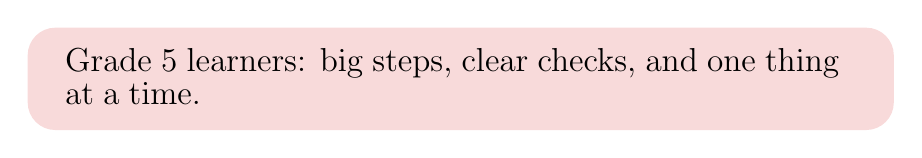
\begin{tikzpicture}
\fill[pbprimary!18, rounded corners=10pt] (0,0) rectangle (11,1.3);
\node[anchor=west, text width=10.2cm] at (0.35,0.68) {\large Grade 5 learners: big steps, clear checks, and one thing at a time.};
\end{tikzpicture}
\end{center}
\end{frame}
\begin{frame}{Todays Goal}
\begin{itemize}
\item I can follow the lesson steps and stay with the class routine.
\item I can try, test, and improve my work.
\item I can show one piece of evidence that I learned something new.
\end{itemize}
\begin{block}{Remember}
We do not have to be perfect right away. We take one step, then the next step, then we check.
\end{block}
\end{frame}
\begin{frame}{What You Need}
\begin{itemize}
\item Your class materials
\item The digital tool or build materials for today
\item A partner voice and your thinking
\end{itemize}
\begin{block}{Partner Norms}
Look. Listen. Try. Talk. Help without taking over.
\end{block}
\end{frame}
\begin{frame}{Step 1}
\begin{block}{Set up the robot and agree on partner roles.}
Set up the robot and agree on partner roles.
\end{block}
\begin{itemize}
\item One partner drives the device, one partner notices what to fix, then switch.
\item Assign partner roles before materials come out so turn-taking is visible.
\end{itemize}
\centering\large\color{pbprimary} Pause. Check. Then move on.
\end{frame}
\begin{frame}{Step 2}
\begin{block}{Build or code one move sequence at a time.}
Build or code one move sequence at a time.
\end{block}
\begin{itemize}
\item Test one change before adding another.
\item Model one test-revise cycle with the actual robot or kit students will use.
\end{itemize}
\centering\large\color{pbprimary} Pause. Check. Then move on.
\end{frame}
\begin{frame}{Step 3}
\begin{block}{Revise after each test and explain your choice.}
Revise after each test and explain your choice.
\end{block}
\begin{itemize}
\item Use We changed this because...
\item Use a simple data language such as what changed, what happened, and what to try next.
\end{itemize}
\centering\large\color{pbprimary} Pause. Check. Then move on.
\end{frame}
\begin{frame}{If You Get Stuck}
\begin{enumerate}
\item Read the directions on your screen or slide one more time.
\item Check the example, the checklist, or your partner role.
\item Try one small change before asking for a full rescue.
\item Device-to-robot pairing and setup can split attention quickly.
\end{enumerate}
\begin{alertblock}{Help Routine}
Stop. Breathe. Point to where you are stuck. Ask a specific question.
\end{alertblock}
\end{frame}
\begin{frame}{Show Your Learning}
\begin{itemize}
\item I stayed with the steps and used the help routine when I needed it.
\item I made, coded, explained, or revised something that matches the lesson goal.
\item I can point to one choice, fix, or idea I learned today.
\end{itemize}
\begin{block}{Before You Leave}
Save it, share it, explain it, or demonstrate it.
\end{block}
\end{frame}
\begin{frame}{Teacher Voiceover Cues}
\footnotesize
\begin{itemize}
\item Today we are working on robot logic and conditional coding. Watch first, then try it with me.
\item If you feel stuck, stop at the checkpoint slide and use the help routine before you panic.
\item Show what you learned by saving, sharing, explaining, or demonstrating one clear success move.
\end{itemize}
\color{gray}This slide can be removed before student use if you only want the visual deck.
\end{frame}
\end{document}
